\documentclass[a4paper, 12pt]{article}%тип документа

%отступы
\usepackage[left=2cm,right=2cm,top=2cm,bottom=3cm,bindingoffset=0cm]{geometry}
\setlength{\parindent}{5ex}

%Русский язык
\usepackage[T2A]{fontenc} %кодировка
\usepackage[utf8]{inputenc} %кодировка исходного кода
\usepackage[english,russian]{babel} %локализация и переносы

%Вставка картинок
\usepackage{graphicx}
\graphicspath{{pictures/}}
\DeclareGraphicsExtensions{.pdf,.png,.jpg}

%Графики
\usepackage{pgfplots}
\pgfplotsset{compat=1.9}

%Математика
\usepackage{amsmath, amsfonts, amssymb, amsthm, mathtools}

%Таблицы
\usepackage{longtable} 
\usepackage{float}

%Римские цифры
\newcommand{\RomanNumeralCaps}[1]{\uppercase\expandafter{\romannumeral#1}}

\usepackage{multirow}


\begin{document}
	\begin{titlepage}
		\begin{center}
			\textsc{Федеральное государственное автономное образовательное учреждение высшего образования«Московский физико-технический институт (национальный исследовательский университет)»\\[5mm]
			}
			
			\vfill
			
			\textbf{Отчёт по лабораторной работы 3.2.5\\[3mm]
				Вынужденные колебания в электрическом контуре
				\\[50mm]
			}
			
		\end{center}
		
		\hfill
		\begin{minipage}{.5\textwidth}
			Выполнил студент:\\[2mm]
			Сериков Василий Романович\\[2mm]
			группа: Б03-102\\[5mm]
			
		\end{minipage}
		\vfill
		\begin{center}
			Москва, 2022 г.
		\end{center}
		
	\end{titlepage}
	
	\newpage
	\textbf{Аннотация}\\
	
	
	\textbf{Цель работы: }\\
	
	Исследование вынужденных колебаний и процессов их установления в колебательном контуре.\\
	
	\textbf{В работе используются: }\\
	
	Генератор звуковых частот, вольтметр, частотомер, конденсатор, катушка индуктивности, магазин сопротивлений, осциллограф, универсальный измеритель импеданса (LCR-метр).\\
	
	\textbf{Теоретические сведения: } \\
	
	При подключении к контуру внешнего синусоидального источника в
	нём возникают колебания, которые можно представить как суперпозицию двух синусоид: первая — с частотой собственных колебаний
	контура и амплитудой, экспоненциально убывающей со временем; вторая — с частотой внешнего источника и постоянной амплитудой. Со временем собственные колебания затухают, и в контуре устанавливаются
	вынужденные колебания. Амплитуда этих колебаний максимальна при
	резонансе: совпадении или достаточной близости частоты внешнего сигнала и собственной частоты контура. Зависимость амплитуды установившихся колебаний от частоты внешнего сигнала называется резонансной
	кривой.
	
	\textbf{А. Резонансная кривая колебательного контура}\\
	Для экспериментального исследования резонансной кривой тока в
	параллельном колебательном контуре используется схема, представленная на рис. 1. Синусоидальный сигнал с генератора подаётся на параллельный колебательный контур через небольшую разделительную ёмкость C1. Напряжение с конденсатора контура C поступает на вертикальный вход электронного осциллографа (ЭО). Для регистрации резонансной кривой необходимо, чтобы модули импедансов возбуждающей Zист и измеряющей Zизм цепей намного превосходили модуль импеданса самого контура вблизи резонанса Zрез = l/RC. С этой целью разделительная ёмкость C1 выбирается
	
	\begin{figure}[h]
		\center{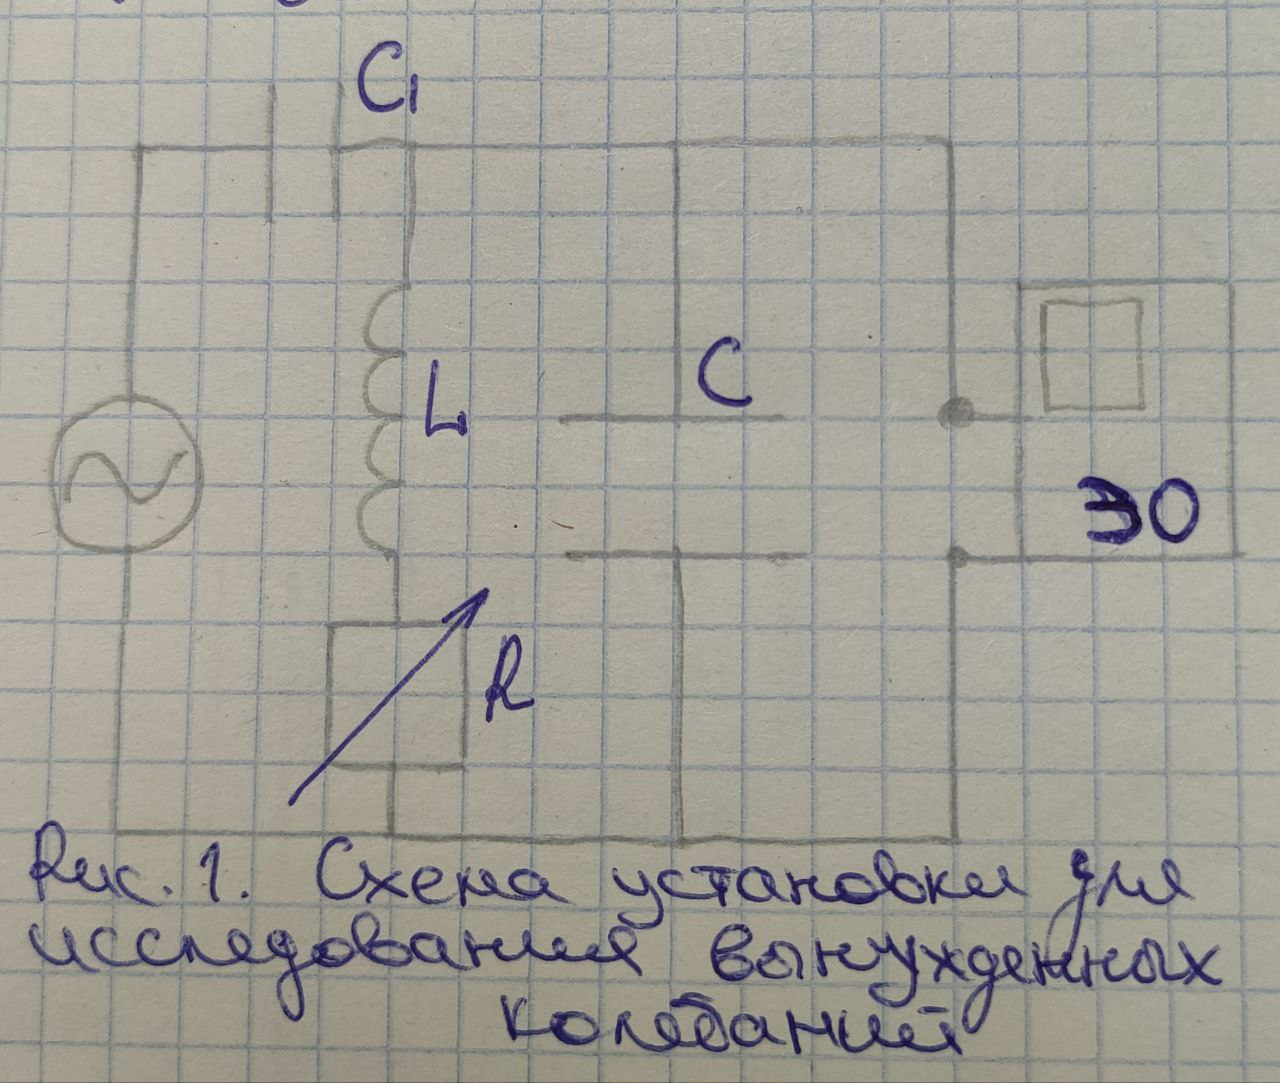
\includegraphics [scale=0.17]{photo2.png}}
	\end{figure}
	
	\newpage
	
	настолько малой, что в рабочем диапазоне частот модуль её импеданса
	$|ZC_1|$ = 1/$\omega C_1$ много больше модуля импеданса контура на частоте $\omega$.
	Таким образом, амплитуда тока в цепи генератора определяется импедансом |$ZC_1|$. Эта амплитуда относительно мало меняется в пределах резонансной кривой колебательного контура, что, однако, приводит к некоторому искажению последней по сравнению со случаем,  где в качестве генератора предполагается источник тока, обладающий большим и постоянным внутренним сопротивлением во всём исследуемом частотном диапазоне. Входное сопротивление осциллографа (измеряющей цепи) достаточно велико: $|Zизм| \approx Rэо \approx$ 1 МОм, поэтому его влиянием можно пренебречь.
	
	
	$$ I_c(\omega) = I(\omega) \sqrt{\frac{1 + Q_m^2(\omega/\omega_0)^2}{1 + Q_m^2(\omega/\omega_0 - \omega_0/\omega)^2}}$$
	
	
	Из соотношения выше следует, что на собственной частоте $\omega_0$ ток в
	высокодобротном контуре почти в Q $>>$ 1 раз превосходит ток во внешней цепи. Именно по этой причине резонанс в параллельном контуре
	называется резонансом токов.\\
	
	
	\textbf{Экспериментальная установка: }\\
	Схема установки для исследования вынужденных колебаний приведена на рис. 2. Колебательный контур состоит из конденсатора C ёмкостью C, катушки L индуктивностью L и магазина сопротивлений R.
	Синусоидальный сигнал генерируется звуковым генератором (ЗГ), а сигнал, состоящий из отрезков синусоиды (цугов), формируется цифровым
	генератором электрических сигналов произвольной формы или комбинацией генератора синусоидального сигнала звукового диапазона и электронного реле, прерывающего сигнал с заданной периодичностью.
	
	Эффективное значение тока $I(\omega)$, текущего к контуру от генератора в режиме непрерывного сигнала, измеряется амперметром A, а
	соответствующее значение тока в контуре определяется по формуле
	$IC(\omega) = \omega CU_C(\omega)$, где $U_C(\omega)$ — эффективное напряжение на конденсаторе, измеряемое вольтметром V.
	
	\begin{figure}[h]
		\center{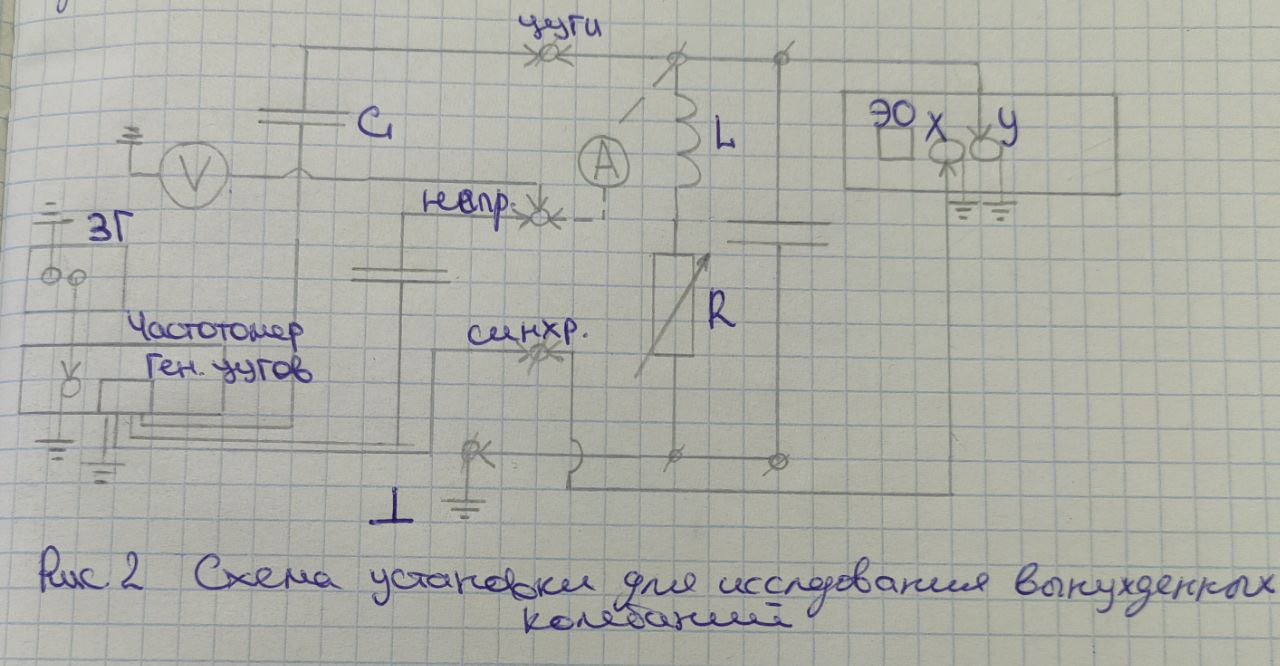
\includegraphics [scale=0.3]{photo1.png}}
	\end{figure}
	
	\newpage
	
	\textbf{Ход работы и обработка результатов: }\\
	
	\begin{enumerate}
		
		\item Рассчитаем собственную частоту: $\nu_0 = 1 / 2 \pi \sqrt{LC} =  1591,5$ Гц
	
		\item Меняя частоту генератора в обе стороны от резонансной, получим зависимость показаний вольтметра V от частоты
		сигнала $\nu$. Полученные данные для различных сопротивлений занесем в таблицу 1. По полученным данным построим графики зависимости $\frac{U}{U_0}(\frac{\nu}{\nu_0})$
		
		\begin{longtable} {|c|c|c|c|c|c|c|c|c|c|c|c|}
			\hline
			\multirow{4}{*}{R = 0 Ом $\searrow$}& $\nu$, Гц & 1567 & 1557 & 1552 & 1548 & 1543 & 1540 & 1535 & 1531 & 1526 & 1522  \\ \cline{2-12}
			&U$\cdot 30$, мВ& 9,8 & 9,5 & 9 & 8,5 & 7,8 & 7,4 & 6,8 & 6,4 & 5,8  & 5,4  \\ \cline{2-12}
			
			& $\nu$, Гц &  1514 & 1505 & 1499 & 1493& 1489&&&&&\\ \cline{2-12}
		   	&U$\cdot 30$, мВ&  4,6 & 4,2& 3,8& 3,5 & 3,4 &&&&& \\ \hline
				 
			\multirow{4}{*}{R = 0 Ом $\nearrow$}& $\nu$, Гц & 1563 & 1574 & 1579 & 1585 & 1588 & 1590 & 1592 & 1597 & 1600 & 1604 \\ \cline{2-12}
			&U$\cdot 30$, мВ& 9,8 & 9,5 & 9 & 8,4 & 8 & 7,7 & 7,4 & 7,0 & 6,6  & 6,2  \\ \cline{2-12}
		
			& $\nu$, Гц  & 1608 & 1615 & 1625 & 1641& 1648&&&&& \\ \cline{2-12}
			&U$\cdot 30$, мВ& 5,8 & 5,2& 4,6& 3,8 & 3,5 &&&&&\\ \hline
			
			
			\hline
			
			\multirow{4}{*}{R = 100 Ом $\searrow$}& $\nu$, Гц &1573& 1547 & 1525 & 1518 & 1498 & 1487 & 1474 & 1462 & 1451 & 1430   \\ \cline{2-12}
			&U$\cdot 30$, мВ&10& 9,7 & 9,2 & 9 & 8,4 & 7,9 & 7,4 & 6,8 & 6,5 & 5,8   \\ \cline{2-12}
			& $\nu$, Гц & 1420& 1390 & 1370 & 1352 & 1316&&&&&\\ \cline{2-12}
			&U$\cdot 30$, мВ& 5,5 & 4,7 & 4,2& 3,9 & 3,4 &&&&& \\ \hline
			
			\multirow{4}{*}{R = 100 Ом $\nearrow$ }& $\nu$, Гц &1573& 1602 & 1612 & 1635 & 1647 & 1672 & 1685 & 1703 & 1727 & 1750   \\ \cline{2-12}
			&U$\cdot 30$, мВ&10& 9,7 & 9,3 & 8,8 & 8,5 & 7,8 & 7,4 & 6,9 & 6,4 & 5,9   \\ \cline{2-12}
			& $\nu$, Гц & 1795& 1829 & 1862 & 1945 & 2058&&&&&\\ \cline{2-12}
			&U$\cdot 30$, мВ& 5,2 & 4,8 & 4,4& 3,8 & 3,4 &&&&& \\ \hline
			\caption{Полученные данные для напряжения и частоты.}
			
		\end{longtable}
		\begin{figure}[H]
			\center{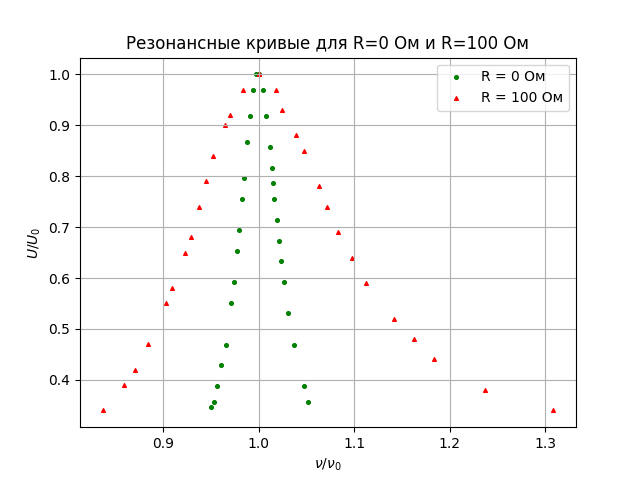
\includegraphics [scale=0.7]{graph_1.png}}
			\caption{График зависимости $\frac{U}{U_0}(\frac{\nu}{\nu_0})$}
		\end{figure}
		
		
		\item Определим добротность по формуле $Q = \nu_0/\delta_{\nu}$, где $\delta_{\nu}$ — ширина резонансной кривой на уровне 0,707.
		
		
		$$ Q_{100} = 6,849 \pm 0,009$$
		$$ Q_0 = 24,39\pm 0,03 $$
		
		\item Для расчёта добротности по скорости нарастания и затухания амплитуды измерим амплитуды двух колебаний $U_k, U_{k+n}$ и амплитуду установившихся колебаний $U_{\infty}$
		
		
		\begin{longtable}{|c|c|c|c|c|c|c|c|c|}  \hline
			{} & \multicolumn{4}{|c|}{$\nearrow$} & \multicolumn{4}{|c|}{$\searrow$} \\\hline
			$U_k,\ \text{дел}$ & 0,4 & 1,4 & 2,2 & 3 & 0,6 & 0,8 & 3 & 4,7 \\\hline
			$U_{k+n}, \text{дел}$ & 3 & 3,6 & 4,8 & 5,6 & 1 & 2,1 & 4,2 & 6 \\\hline
			$n$ & 3 & 3 & 4 & 5 & -4 & -8 & -3 & -2 \\\hline
			$Q$ & 21,40 & 21,94 & 19,63 & 19,50 & 24,60 & 26,04 & 26,68 & 25,73 \\\hline
			\caption{Данные нарастаний и затуханий цуги при $R = 0\ \text{Ом, } U_{\infty} = 7,7$ дел}
		\end{longtable}
		
		
		\begin{longtable}{|c|c|c|c|c|c|c|c|c|}  \hline
			{} & \multicolumn{4}{|c|}{$\nearrow$} & \multicolumn{4}{|c|}{$\searrow$} \\\hline
			$U_k,\ \text{дел}$ & 2,2 & 4,1 & 5,5 & 6,4 & 0,2 & 0,4 & 1,8 & 4,2 \\\hline
			$U_{k+n}, \text{дел}$ & 4,1 & 5,5 & 6,4 & 7 & 0,9 & 1,2 & 2,7 & 6,5 \\\hline
			$n$ & 1 & 1 & 1 & 1 & -4 & -3 & -1 & -1 \\\hline
			$Q$ & 7,58 & 6,61 & 6,33 & 5,61 & 8,35 & 8,58 & 7,74 & 7,46 \\\hline
			\caption{Данные нарастаний и затуханий цуги при $R = 100\ \text{Ом, } U_{\infty} = 7,8$ дел}
		\end{longtable}
		
		$$  Q_{\text{затухания}} = \frac{\pi}{\Theta} = \pi (\frac{1}{n} \ln \frac{U_k}{U_{k+n}})^{-1}  $$
		
		$$ Q_{\text{нарастания}} = \frac{\pi}{\Theta} =  \pi (\frac{1}{n} \ln \frac{U_0 - U_k}{U_0 - U_{k+n}})^{-1}  $$
		
		\item Измерим активное сопротивление $R_L$ и индуктивность L магазина
		индуктивностей с помощью измерителя импедансов на частотах 50 Гц, 500 Гц и 1500 Гц. Данные занесем в таблицу 4.
		
		$$ Q = \frac{1}{R}\sqrt{\frac{L}{C}} $$
		
		\begin{longtable} {|c|c|c|c|}
			\hline
			 $\nu$, Гц &  $R_L$, Ом & $L$, мГн & $C$, мкФ \\ \hline
			50 & 29,3 & 99,9 & 101,3 \\ \hline
			500 & 29,5 & 99,8 & 1,0 \\ \hline
			1500 & 30,4 & 99,5 & 0,1 \\ \hline
			\caption{Данные, полученные с LCR-метра}
		\end{longtable}
		
	\item Сведем полученные данные для Q в одну таблицу, где $R_{\Sigma} = R + R_L$
	
		\begin{longtable} {|c|c|c|c|c|c|}
		\hline
		\multirow{2}{*}{R, Ом} & 	\multirow{2}{*}{$R_{\Sigma}, $ Ом} & \multicolumn{4}{|c|}{Q} \\ \cline{3-6}
		& & Ширина кривой & Нарастание & Затухание & $f(RLC)$ \\\hline
		
		0 & 30,4 & 24,39 $\pm 0,03$ & 20,6 $\pm 0,3$& 25,8 $\pm 0,5$& 32,8$\pm 0,1$ \\\hline
		100 & 130,4 & 6,849 $\pm 0,009$ & 6,5 $\pm 0,1$& 8,0$\pm 0,2$ & 7,67$\pm 0,02$\\\hline
		
		\caption{Сводная таблица для Q}
		\end{longtable}
		
		
	\end{enumerate}
	
	
	\textbf{Обсуждение результатов и выводы: }\\
	
	В данной работе мы исследовали вынужденные колебания и процессы их установления в колебательном контуре.
	
	Получили зависимости для построения резонансной кривой, посчитали значения добротность системы различными способами: по ширине резонансной кривой, по нарастанию амплитуды, по затуханию амплитуды, по теоретическому значению добротности через параметры
	контура L, C и R. Полученные значения отличаются друг от друга, так как в каждом способе есть свои приближения.
	
	
	
	
	
	
	
	
\end{document}